%# -*- coding: utf-8-unix -*-
%% app2.tex for SJTU Master Thesis
%% based on CASthesis
%% modified by wei.jianwen@gmail.com
%% version: 0.3a
%% Encoding: UTF-8
%% last update: Dec 5th, 2010
%%==================================================

\chapter{相关公式}
\begin{section}{变异系数}
 标准差与平均数的比值称为变异系数,又称“离散系数",记为C.V。变异系数主要用于在单位和(或)平均数不同时对两个或多个资料变异程度比较。用以下公式计算:
\begin{equation}
    C.V = \frac{\sigma }{\mu }
\end{equation}
其中$\sigma$是标准差,而$\mu$是平均值。
\end{section}


\begin{section}{劳伦茨曲线}
劳伦茨曲线是经济学家马克斯·劳伦茨在1905年提出的表示收入分配的曲线.在经济学中,劳伦兹曲线是在过往财富分配数据上建立的累积分布函数所对应的曲线,该曲线通过变量y\%的值来反映各项分配的比例。劳伦茨曲线经常被用来描述收入的分配情况,即用x\%代表一部分家庭占整个社会家庭的比例,以y\%代表该部分家庭的总收入占整个社会总收入的比例。图\ref{Fig:GN}是一个劳伦茨曲线示例。
\end{section}


\begin{section}{基尼系数}
基尼系数是20世纪初意大利学者科拉多·基尼在劳伦茨曲线的基础上所定义的判断年收入分配公平程度的指标。基尼系数是比例数据,介于0和1之间。基尼系数越小,年收入分配越平均,基尼系数越大,年收入分配越不平均。设图\ref{Fig:GN}中的实际收入分配曲线(红线)和收入分配绝对平等线(绿线)之间的面积为A,实际收入分配曲线(红线)和收入分配绝对不平等线(蓝线)之间的面积为B,则表示收入与人口之间的比例的基尼系数可以表示为
\begin{equation}
    G = \frac{A }{A+B }
\end{equation}

\end{section}

\begin{figure}[H]
	\centering
	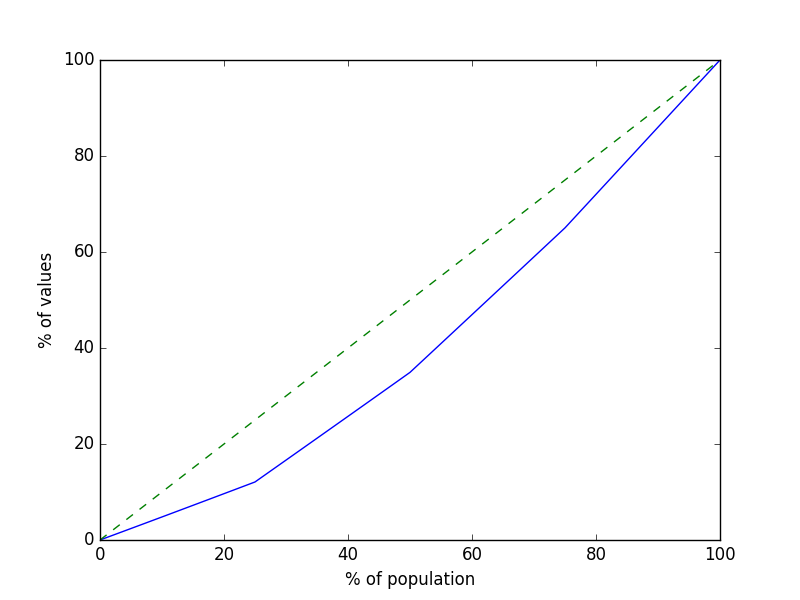
\includegraphics[width=5.0in]{GN.png}
	\caption{劳伦茨曲线示例}
	\label{Fig:GN}
\end{figure}
